\documentclass[aspectratio=169]{beamer}
\usetheme{metropolis}
\usepackage{booktabs}
\usepackage{amsmath,amssymb}
\usepackage{listings}
\usepackage{tikz}
\usetikzlibrary{positioning,arrows.meta,calc}

\lstset{
  basicstyle=\ttfamily\scriptsize,
  keywordstyle=\color{blue},
  commentstyle=\color{gray},
  breaklines=true,
  frame=none,
}

\newcommand{\FF}{\mathcal{F}}
\newcommand{\Hom}{\mathrm{Hom}}
\newcommand{\R}{\mathbb{R}}
\newcommand{\Z}{\mathbb{Z}}
\newcommand{\C}{\mathbb{C}}
\newcommand{\SO}{\mathrm{SO}}
\newcommand{\Ind}{\mathrm{Ind}}

\title{The Steerable Bispectrum for Non-Abelian Groups}
\subtitle{Bridging Equivariant Networks and Complete Invariant Theory}
\author{Johan Mathe}
\date{\today}

\begin{document}

\maketitle

\begin{frame}{Two worlds, one gap}
  \begin{columns}[T]
    \begin{column}{0.47\textwidth}
      \textbf{Steerable CNNs}\\
      {\small Weiler \& Cesa 2019}

      \medskip

      \begin{itemize}\small
        \item Equivariant by design
        \item Learned filters on intertwiner basis
        \item Invariance via \alert{norm / gated nonlinearities}
        \item[$\to$] Discards phase information
        \item[$\to$] No reconstruction guarantees
      \end{itemize}
    \end{column}
    \begin{column}{0.47\textwidth}
      \textbf{$G$-Bispectrum}\\
      {\small Kakarala 1992, Mataigne et al.\ 2024}

      \medskip

      \begin{itemize}\small
        \item Complete invariant (up to group action, under non-degeneracy)
        \item Signal recoverable from bispectrum (generically)
        \item Selective: $O(|G|)$ instead of $O(|G|^2)$ coefficients
        \item[$\to$] Requires \alert{proper Fourier coefficients}
        \item[$\to$] Not embedded in learned architectures
      \end{itemize}
    \end{column}
  \end{columns}

  \bigskip
  \centering
  \alert{Gap}: What seems to be missing is a principled identification between steerable\\
  feature coefficients and the Fourier objects required by the non-abelian bispectrum.
\end{frame}

\begin{frame}{What does ``steerable'' mean?}
  A basis of filter functions is \textbf{steerable} if group actions reduce to linear operations on the coefficients:
  \[
    \mathbf{Y}(g \cdot x) = \rho(g) \, \mathbf{Y}(x)
  \]
  where $\mathbf{Y}$ is vector-valued and $\rho(g)$ is a matrix representation.

  \medskip

  \begin{columns}[T]
    \begin{column}{0.48\textwidth}
      \textbf{Abelian} ($\SO(2)$, $C_n$):\\
      Each basis element $Y_l$ transforms by a \textit{scalar} character: $Y_l(g \cdot x) = \chi_l(g) \, Y_l(x)$.\\
      {\small E.g.\ $e^{ik\theta} \mapsto e^{ik\phi} \cdot e^{ik\theta}$}
    \end{column}
    \begin{column}{0.48\textwidth}
      \textbf{Non-abelian} ($D_n$, $O$):\\
      Basis elements within an isotypic block \textit{mix} under the group action via a matrix $\rho(g)$.\\
      {\small E.g.\ the 2D irrep $E$ of $D_4$}
    \end{column}
  \end{columns}

  \bigskip

  \textbf{Analogy}: a spotlight on a gimbal. You turn a dial (apply $\rho(g)$) and the beam rotates analytically --- no grid resampling.

  \medskip

  {\small Reference: Freeman \& Adelson, \textit{The Design and Use of Steerable Filters}, IEEE TPAMI 1991.}
\end{frame}

\begin{frame}{What is the bispectrum?}\small
  \textbf{Abelian case} ($C_n$, $\SO(2)$): scalar triple product
  \vspace{-4pt}
  \[
    \beta_{k_1, k_2} = \hat{f}_{k_1} \cdot \hat{f}_{k_2} \cdot \hat{f}^*_{k_1 + k_2}
  \]

  \vspace{-6pt}

  \textbf{Non-abelian case} ($D_n$, $O$, $\SO(3)$): schematic CG-based formula
  \vspace{-4pt}
  \[
    \beta_{\rho_1, \rho_2} = \bigl[\FF_{\rho_1} \otimes \FF_{\rho_2}\bigr]
    \, C_{\rho_1,\rho_2} \, \Bigl[\bigoplus_{\rho \in \rho_1 \otimes \rho_2} \FF_\rho^\dagger\Bigr] \, C_{\rho_1,\rho_2}^\dagger
  \]

  \vspace{-6pt}

  {\scriptsize where $\FF_\rho$ denotes the matrix-valued Fourier coefficient at irrep $\rho$, and $C_{\rho_1,\rho_2}$ is the CG change-of-basis for $\rho_1 \otimes \rho_2$.}

  \medskip

  \textbf{Key property}: under standard non-degeneracy assumptions (invertibility of relevant Fourier blocks), the bispectrum is a \textit{complete} invariant --- it recovers $f$ up to group action. The power spectrum $|\hat{f}_k|^2$ is not (loses phase).

  \medskip

  \textbf{Selective bispectrum} (Mataigne et al.\ 2024): only $O(|G|)$ coefficients needed instead of $O(|G|^2)$, preserving completeness.
\end{frame}

\begin{frame}{Timeline: two parallel lines of work}
  \centering
  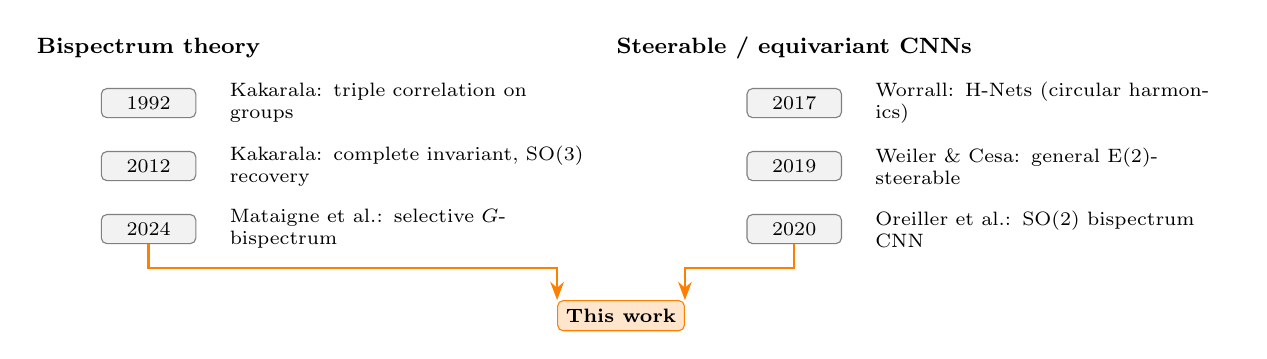
\begin{tikzpicture}[
    node distance=0.3cm and 0.8cm,
    every node/.style={font=\scriptsize},
    yearbox/.style={rounded corners=2pt, draw=gray, fill=gray!10, inner sep=3pt, minimum width=1.2cm},
    paper/.style={align=left, text width=4.5cm},
    >=Stealth
  ]
    \node[font=\footnotesize\bfseries] (bisp_label) at (-3, 2.2) {Bispectrum theory};
    \node[yearbox] (k92) at (-3, 1.5) {1992};
    \node[paper, right=0.3cm of k92] {Kakarala: triple correlation on groups};
    \node[yearbox] (k12) at (-3, 0.7) {2012};
    \node[paper, right=0.3cm of k12] {Kakarala: complete invariant, SO(3) recovery};
    \node[yearbox] (m24) at (-3, -0.1) {2024};
    \node[paper, right=0.3cm of m24] {Mataigne et al.: selective $G$-bispectrum};

    \node[font=\footnotesize\bfseries] (steer_label) at (5.2, 2.2) {Steerable / equivariant CNNs};
    \node[yearbox] (w17) at (5.2, 1.5) {2017};
    \node[paper, right=0.3cm of w17] {Worrall: H-Nets (circular harmonics)};
    \node[yearbox] (w19) at (5.2, 0.7) {2019};
    \node[paper, right=0.3cm of w19] {Weiler \& Cesa: general E(2)-steerable};
    \node[yearbox] (o20) at (5.2, -0.1) {2020};
    \node[paper, right=0.3cm of o20] {Oreiller et al.: SO(2) bispectrum CNN};

    \node[yearbox, fill=orange!20, draw=orange] (ours) at (3, -1.2) {\textbf{This work}};
    \draw[->, thick, orange] (m24.south) -- ++(0, -0.3) -| (ours.north west);
    \draw[->, thick, orange] (o20.south) -- ++(0, -0.3) -| (ours.north east);
  \end{tikzpicture}
\end{frame}

\begin{frame}{}
  \vfill
  \centering
  {\Large\textbf{Part I: The Abelian Case}}

  \medskip

  {\normalsize How the steerable bispectrum works for $\SO(2)$}
  \vfill
\end{frame}

\begin{frame}{$\SO(2)$ steerable bispectrum}
  \textbf{Filter}: $\Psi_k(r, \theta) = w_k(r) \cdot e^{ik\theta}$ \quad (learned radial profile $\times$ circular harmonic)

  \medskip

  \textbf{Convolution}: produces per-pixel steerable coefficients $\hat{\Theta}_k$

  \medskip

  \textbf{Steerability}: rotate input by $\phi$ $\Rightarrow$ $\hat{\Theta}_k \mapsto e^{ik\phi} \hat{\Theta}_k$

  \medskip

  \textbf{Bispectrum}: triple product cancels the phase
  \[
    \beta_{k_1, k_2} = \hat{\Theta}_{k_1} \cdot \hat{\Theta}_{k_2} \cdot \hat{\Theta}^*_{k_1+k_2}
  \]
  since $e^{ik_1\phi} \cdot e^{ik_2\phi} \cdot e^{-i(k_1+k_2)\phi} = 1$.

  \bigskip

  This is the same scalar triple-product mechanism as \texttt{CnonCn}, applied per-pixel to circular-harmonic responses.

  \medskip

  \textbf{Why it works}: $\SO(2)$ is abelian $\Rightarrow$ all irreps are 1D characters $\Rightarrow$ scalar steerable coordinates align with scalar Fourier modes.
\end{frame}

\begin{frame}[fragile]{The existing implementation (Oreiller et al.\ 2022)}
  The \texttt{BCHConv2D} layer in \texttt{voreille/2d\_bispectrum\_cnn}:

  \begin{lstlisting}[language=Python]
def call(self, inputs):
    x = self.conv_ch(inputs)     # circular harmonic convolution
    outputs = list()
    for n1, n2 in self.indices:
        bispectrum = (x[..., n1] * x[..., n2] *
                      tf.math.conj(x[..., n1 + n2]))
        outputs.append(tf.math.real(bispectrum))
        if n1 != 0:
            outputs.append(tf.math.imag(bispectrum))
    x = tf.concat(outputs, axis=-1)
  \end{lstlisting}

  \medskip

  \begin{itemize}
    \item TensorFlow/Keras, not PyTorch
    \item Redundant index set (${\sim}n^2/2$ pairs via symmetry reduction)
    \item No selectivity, no inversion guarantees
    \item Learned discrete radial profiles (pixel masks), not Fourier-Bessel basis
  \end{itemize}
\end{frame}

\begin{frame}{What's missing for the $\SO(2)$ case}
  \begin{table}
    \scriptsize
    \begin{tabular}{lccc}
      \toprule
      & \textbf{Oreiller et al.} & \textbf{Our library} & \textbf{Potential} \\
      \midrule
      Bispectral pairs & ${\sim}n^2/2$ (symmetry) & $n$ (selective) & Same accuracy, fewer channels \\
      Inversion & None & \checkmark\ (bootstrap) & Reconstruct from invariants \\
      Radial basis & Learned pixel masks & Bessel $J_n(\lambda_{nk}r)$ & Orthogonal, complete \\
      Framework & TensorFlow & PyTorch & GPU-optimized \\
      \bottomrule
    \end{tabular}
  \end{table}

  \bigskip

  At $n_\text{harmonics} = 4$: selective gives 4 vs their 6 coefficients --- negligible.

  \medskip

  At $n_\text{harmonics} = 32$: selective gives 32 vs ${\sim}528$ coefficients.

  \medskip

  At $n_\text{harmonics} = 64$: selective gives 64 vs ${\sim}2080$ coefficients.

  \bigskip

  Selectivity matters when angular resolution is high, and becomes critical in 3D where full bispectral constructions scale poorly with harmonic bandwidth.
\end{frame}

\begin{frame}{Why the abelian case is easy}
  For an abelian group $G$, all irreps are 1D characters $\chi_k : G \to \C$.

  \medskip

  The intertwiner space $\Hom^G(\pi, \chi_k)$ has dimension equal to the multiplicity of $\chi_k$ in $\pi$.

  \medskip

  For the regular representation on $\Z/n\Z$: every character appears exactly once.

  \bigskip

  In the regular abelian case, the equivariant decomposition coincides with the Fourier decomposition: every irrep is 1D, appears once, and $L = M = n$.

  \bigskip

  Hence the steerable coefficients $\hat{\Theta}_l$ can be identified with the Fourier coefficients $\hat{f}_l$.

  \medskip

  $\Rightarrow$ The standard bispectrum formula applies directly.

  \bigskip

  \alert{For non-abelian groups, the simple scalar identification between steerable coefficients and Fourier coefficients breaks.}
\end{frame}

\begin{frame}{}
  \vfill
  \centering
  {\Large\textbf{Part II: The Non-Abelian Problem}}

  \medskip

  {\normalsize Why $L \neq M$ blocks the standard approach}
  \vfill
\end{frame}

\begin{frame}{The $L \neq M$ problem}
  Consider $H = D_4$ with a \textbf{trivial output representation} $\rho_0$.

  \medskip

  A trivial-output head accesses only the $A_1$-isotypic component of the input fiber $\pi$. But $D_4$ has $M = 5$ irreps: $A_1, A_2, B_1, B_2, E$ (dims $1,1,1,1,2$).

  \bigskip

  {\small Count-of-types intuition (not a dimensional comparison):}

  \centering\small
  \begin{tabular}{lcl}
    \toprule
    & Irreps accessed by trivial output & Total irreps of $H$ \\
    \midrule
    $\SO(2)$, $C_n$ (abelian) & all $n$ (each 1D) & $n$ \\
    $D_4$, $\rho = \rho_0$ & \alert{$A_1$ only} & \alert{5 (incl.\ 2D $E$)} \\
    $D_8$, $\rho = \rho_0$ & \alert{$A_1$ only} & \alert{7 (incl.\ 2D irreps)} \\
    \bottomrule
  \end{tabular}

  \raggedright

  \bigskip

  The steerable conv gives access only to the \alert{$A_1$-isotypic coordinates}, while the bispectrum requires \alert{Fourier data from all 5 irreps} of $D_4$, including matrix-valued blocks.
\end{frame}

\begin{frame}{Why $L \neq M$}
  The number of intertwiner basis functions is:
  \[
    L = \dim \Hom^H(\pi, \rho) = \sum_{\text{irreps }\psi} m^\pi_\psi \cdot m^\rho_\psi
  \]

  For $\rho = \rho_0$ (trivial): $m^{\rho_0}_\psi = 0$ for all $\psi \neq \rho_0$, so $L = m^\pi_{\rho_0}$.

  \bigskip

  This counts only how many times the \textit{trivial} irrep appears in $\pi$ --- it says nothing about the other irreps.

  \bigskip

  \textbf{The Fourier coefficients $\FF(f)_\psi$} for the non-trivial irreps ($A_2, B_1, B_2, E$) are \textbf{invisible} to a steerable conv with trivial output.

  \bigskip

  \textbf{For abelian groups} in the regular representation: every irrep is 1D and appears with multiplicity one, so the equivariant decomposition aligns with the Fourier decomposition and $L = M$.
\end{frame}

\begin{frame}{What the coefficients actually are}
  The steerable conv produces per-pixel coefficients $\hat{\Theta}_l$, which are projections onto the $\rho_0$\textbf{-isotypic component} of the input fiber $\pi$:

  \begin{itemize}
    \item \textbf{Visible} through a trivial-output head: the $A_1$-isotypic component, of multiplicity $m^{\pi}_{A_1} = 3$
    \item \alert{Not visible} through a trivial-output head: the $A_2, B_1, B_2, E$ isotypic components (4 irreps, including the matrix-valued $E$ block)
  \end{itemize}

  \bigskip

  $\Rightarrow$ The bispectrum computed from $\hat{\Theta}_l$ alone is \textit{incomplete}.

  \medskip

  $\Rightarrow$ For a complete invariant, we need Fourier data for \alert{all} irreps $\FF_\psi$.
\end{frame}

\begin{frame}{Information flow: the problem and our solution}
  \centering
  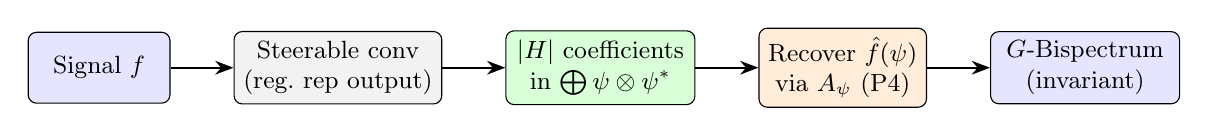
\begin{tikzpicture}[
    box/.style={draw, rounded corners=3pt, minimum height=0.9cm, font=\small, align=center},
    >=Stealth,
    node distance=0.5cm
  ]
    \node[box, fill=blue!10, minimum width=1.8cm] (sig) {Signal $f$};
    \node[box, fill=gray!10, right=0.8cm of sig, minimum width=2.4cm] (conv) {Steerable conv\\(reg.\ rep output)};
    \node[box, fill=green!15, right=0.8cm of conv, minimum width=2.4cm] (coef) {$|H|$ coefficients\\in $\bigoplus \psi \otimes \psi^*$};
    \node[box, fill=orange!15, right=0.8cm of coef, minimum width=1.8cm] (inv) {Recover $\hat{f}(\psi)$\\via $A_\psi$ (P4)};
    \node[box, fill=blue!10, right=0.8cm of inv, minimum width=2.4cm] (bisp) {$G$-Bispectrum\\(invariant)};

    \draw[->, thick] (sig) -- (conv);
    \draw[->, thick] (conv) -- (coef);
    \draw[->, thick] (coef) -- (inv);
    \draw[->, thick] (inv) -- (bisp);
  \end{tikzpicture}

  \bigskip

  \begin{tabular}{lll}
    \toprule
    \textbf{Group} & \textbf{Solution} & \textbf{Status} \\
    \midrule
    $\SO(2)$, $C_n$ (abelian) & Identity ($L=M$) & \checkmark\ Solved (Oreiller 2020) \\
    $D_n$ (non-abelian) & Regular-rep fiber + P4 & Proved for model case (this work) \\
    $O$ (octahedral) & Same rep-theoretic construction & Expected to apply \\
    \bottomrule
  \end{tabular}

  \bigskip

  Previously, steerable CNNs for $D_n$ were stuck with \textbf{norm} (loses phase) or \textbf{gated} (ad-hoc). P4 with the regular-rep fiber gives a principled construction and a clear sufficient condition for bispectral pooling.
\end{frame}

\begin{frame}{}
  \vfill
  \centering
  {\Large\textbf{Part III: The Solution}}

  \medskip

  {\normalsize Regular-representation output fiber and Proposition P4}
  \vfill
\end{frame}

\begin{frame}{Construction: regular-representation output fiber}
  \textbf{Key idea}: design the output fiber to be the \textbf{regular representation} of $H$.

  \medskip

  For each irrep $\psi$, the Fourier block $\hat{f}(\psi) \in \psi \otimes \psi^*$ has dimension $d_\psi^2$. To recover it, the $\psi$-typed output needs multiplicity $d_\psi$ (not just 1).

  \medskip

  For $D_4$, the regular representation $\C[D_4] \cong \bigoplus_\psi \psi \otimes \psi^*$ gives:
  \begin{center}\scriptsize
  \begin{tabular}{lccccc}
    \toprule
    Irrep $\psi$ & $d_\psi$ & Canonical mult.\ (reg.\ rep) & Output $\psi \otimes \psi^*$ & Scalar dim & Fourier block \\
    \midrule
    $A_1$ & 1 & 1 & $A_1 \otimes A_1^*$ & 1 & $\hat{f}(A_1) \in \C$ \\
    $A_2$ & 1 & 1 & $A_2 \otimes A_2^*$ & 1 & $\hat{f}(A_2) \in \C$ \\
    $B_1$ & 1 & 1 & $B_1 \otimes B_1^*$ & 1 & $\hat{f}(B_1) \in \C$ \\
    $B_2$ & 1 & 1 & $B_2 \otimes B_2^*$ & 1 & $\hat{f}(B_2) \in \C$ \\
    $E$ & 2 & \alert{2} & $E \otimes E^*$ & \alert{4} & $\hat{f}(E) \in \C^{2\times 2}$ \\
    \midrule
    \textbf{Total} & & & & $8 = |D_4|$ & All 5 Fourier blocks \\
    \bottomrule
  \end{tabular}
  \end{center}

  Total dimension: $1 + 1 + 1 + 1 + 4 = 8 = |D_4|$, recovering all 5 Fourier blocks.
\end{frame}

\begin{frame}{Why multiplicity $d_\psi$ matters}
  \alert{Key}: a single $E$-field (2 scalars) cannot recover the $E$-Fourier block ($2\!\times\!2$ matrix, 4 scalars).

  \bigskip

  You need \textbf{two copies} of $E$, i.e.\ $E \otimes E^* \cong \mathrm{End}(E)$.

  \medskip

  More generally, $\hat{f}(\psi) \in \psi \otimes \psi^*$ has $d_\psi^2$ scalar entries. A $\psi$-typed output with multiplicity $m < d_\psi$ produces only $m \cdot d_\psi$ scalars --- not enough to determine the full Fourier block.

  \bigskip

  The regular representation is the \textit{canonical} choice: it gives each irrep $\psi$ exactly multiplicity $d_\psi$, which is both necessary and sufficient.
\end{frame}

\begin{frame}{Proposition P4 (proved for $V = \C[H]$)}
  \textbf{Proposition.} Let $V = \C[H]$ (regular representation). Let $T_\psi \in \Hom^H(V, \psi \otimes K)$ be an equivariant map with output type $\psi \otimes K$. Then there exists a linear map $A_\psi : \psi^* \to K$ such that
  \[
    T_\psi(f) = (I_\psi \otimes A_\psi) \, \hat{f}(\psi).
  \]
  If $K \cong \psi^*$ and $A_\psi$ is an isomorphism, then $\hat{f}(\psi)$ is linearly recoverable.

  \bigskip

  \textbf{Consequence}: with a regular-rep output fiber ($K = \psi^*$ for each irrep), the steerable conv output is linearly equivalent to the full set of Fourier blocks. Selectivity (Mataigne et al.\ 2024) then applies directly.
\end{frame}

\begin{frame}{Proof of P4 (step 1: decomposition)}\small
  \textbf{Step 1 (Peter--Weyl).} The regular representation decomposes as
  \[
    V = \C[H] \;\cong\; \bigoplus_{\psi \in \widehat{H}} \psi \otimes \psi^*,
  \]
  where each summand $V_\psi = \psi \otimes \psi^*$ is the \textit{$\psi$-isotypic component}, a $d_\psi \times d_\psi$ matrix space. The group acts on the left factor: $h \cdot (u \otimes \lambda) = (\psi(h)u) \otimes \lambda$.

  \medskip

  The orthogonal projection $P_\psi : V \to V_\psi$ is exactly the Fourier transform at $\psi$:
  \[
    P_\psi f \;\longleftrightarrow\; \hat{f}(\psi) = \sum_{g \in H} f(g)\,\psi(g)^* \;\in\; \C^{d_\psi \times d_\psi}.
  \]

  \medskip

  Write $V = V_\psi \oplus V_\psi^\perp$, where $V_\psi^\perp = \bigoplus_{\phi \neq \psi} V_\phi$.
\end{frame}

\begin{frame}{Proof of P4 (step 2: Schur kills wrong frequencies)}\small
  \textbf{Step 2 (Schur's lemma).} The map $T_\psi : V \to \psi \otimes K$ is $H$-equivariant, with the target transforming as $\psi$ in the first factor.

  \medskip

  Restrict $T_\psi$ to a summand $V_\phi = \phi \otimes \phi^*$ with $\phi \neq \psi$. This restriction is an equivariant map $\phi \otimes \phi^* \to \psi \otimes K$. Since $H$ acts on the first factors, this requires an equivariant map $\phi \to \psi$.

  \medskip

  Schur's lemma: if $\phi \not\cong \psi$, every equivariant map $\phi \to \psi$ is \textbf{zero}.

  \medskip

  Therefore $T_\psi$ annihilates $V_\psi^\perp$ and factors through the Fourier projection:
  \[
    T_\psi = \tilde{T}_\psi \circ P_\psi, \qquad \tilde{T}_\psi : \underbrace{\psi \otimes \psi^*}_{= V_\psi} \;\longrightarrow\; \psi \otimes K.
  \]

  \medskip

  \textit{Consequence}: equivariance forces frequency selectivity --- $T_\psi$ can only access the Fourier block $\hat{f}(\psi)$.
\end{frame}

\begin{frame}{Proof of P4 (step 3: structure on the right frequency)}\small
  \textbf{Step 3 (classification of equivariants).} We must classify all $H$-equivariant maps
  \[
    \tilde{T}_\psi : \psi \otimes \psi^* \;\longrightarrow\; \psi \otimes K,
  \]
  where $H$ acts on $\psi$ (first factor) and acts trivially on $\psi^*$ and $K$.

  \medskip

  By Schur's lemma applied to the $\psi$-factor: any equivariant map $\psi \to \psi$ is a scalar multiple of the identity. Therefore $\tilde{T}_\psi$ must act as the identity on the first factor:
  \[
    \tilde{T}_\psi = I_\psi \otimes A_\psi, \qquad A_\psi : \psi^* \to K \;\text{(arbitrary linear map)}.
  \]

  \medskip

  Combining steps 1--3:
  \[
    \boxed{T_\psi(f) = (I_\psi \otimes A_\psi)\,\hat{f}(\psi).}
  \]

  When $K \cong \psi^*$ and $A_\psi$ is invertible, we recover $\hat{f}(\psi) = (I_\psi \otimes A_\psi^{-1})\,T_\psi(f)$. \qed

  \medskip

  \textbf{Remark}: the proof uses only Peter--Weyl and Schur's lemma --- it holds for \textit{any} finite group $H$, not just $D_4$.
\end{frame}

\begin{frame}{Approach 2: direct triple correlation}\small
  \textbf{Idea}: bypass the steerable-to-Fourier identification entirely. Define the triple correlation directly on vector-valued signals with an induced representation action.

  \smallskip

  \textbf{What we have proven} (in our notes):
  \begin{enumerate}\setlength{\itemsep}{1pt}
    \item A triple correlation $T(f)_{g_1, g_2}$ for vector-valued $f$ with action $T_{tr}[f](x) = \rho_H(r) \, f\bigl((tr)^{-1}x\bigr)$.
    \item \textbf{Invariance}: $T(T_h[f]) = T(f)$ for all $h \in H$ (change of variable $r' = rr_h$, $t' = R_h t + t_h$).
    \item \textbf{Bispectrum recovery}: FT of $T(f)$ recovers the standard CG-based bispectrum formula.
  \end{enumerate}

  \smallskip

  This confirms the bispectrum is well-defined for induced-representation signals. In the regular-rep model case, P4 resolves the steerable-to-Fourier identification. For \texttt{escnn}-style induced features over $\R^2$, the identification of the intertwiner basis with the Fourier multiplicity space \alert{remains to be verified}.
\end{frame}

\begin{frame}{Proof status from our derivations}\small
  \vspace{-4pt}
  \begin{center}\scriptsize
  \begin{tabular}{llll}
    \toprule
    \textbf{Result} & \textbf{Status} & \textbf{Where} \\
    \midrule
    TC definition for induced rep & \checkmark Done & Eq.\ in our notes \\
    TC invariance proof & \checkmark Done & Change of variable $r'=rr_h$, $t'=Rt_h+t$ \\
    Bispectrum = FT of TC & \checkmark Done & CG-based derivation \\
    Standard CG formula recovered & \checkmark Done & $\beta = [\FF_{\rho_1} \otimes \FF_{\rho_2}] C [\bigoplus \FF_\rho^\dagger] C^\dagger$ \\
    \midrule
    $\FF_\rho$ from steerable conv (P4) & \checkmark Done & Schur + Peter--Weyl on regular rep \\
    Selectivity transfers & \checkmark Done & Direct from P4 + Mataigne et al. \\
    Channel count: $|H|$ scalars suffice & \checkmark Done & Regular rep has dim $|H|$ \\
    \midrule
    \texttt{escnn} fiber = regular rep & \alert{Open} & Implementation question \\
    \bottomrule
  \end{tabular}
  \end{center}

  \medskip

  \textbf{Remaining question}: the theorem holds for the regular representation. In \texttt{escnn}, the fiber is an architecture choice. The open task is to verify that \texttt{escnn} allows setting the output type to $A_1 \oplus A_2 \oplus B_1 \oplus B_2 \oplus 2E$ and to compute $A_\psi$ from the intertwiner basis.
\end{frame}

\begin{frame}{Selectivity transfers (from P4)}\small
  Since P4 establishes that the steerable conv with regular-rep fiber recovers all Fourier blocks, Mataigne et al.\ (2024) selectivity applies directly:

  \medskip

  \textbf{Channel count per pixel}, for group $H$:

  \vspace{-4pt}
  \begin{center}\scriptsize
  \begin{tabular}{lccc}
    \toprule
    \textbf{Invariant} & \textbf{Channels} & \textbf{Complete?}$^\dagger$ & \textbf{Invertible?}$^\dagger$ \\
    \midrule
    Norm (power spectrum) & $O(|H|)$ & No & No \\
    Full bispectrum & $O(|H|^2)$ & Yes & Yes \\
    \textbf{Selective bispectrum} & $\boldsymbol{O(|H|)}$ & \textbf{Yes} & \textbf{Yes} \\
    \multicolumn{4}{l}{\tiny $^\dagger$Under standard non-degeneracy assumptions (Kakarala 1992, Mataigne et al.\ 2024).}\\
    \bottomrule
  \end{tabular}
  \end{center}

  \vspace{-2pt}

  Concrete numbers for $D_n$:

  \vspace{-4pt}
  \begin{center}\scriptsize
  \begin{tabular}{lrrr}
    \toprule
    Group & $|H|$ & Full bisp.\ channels & Selective channels \\
    \midrule
    $D_4$ & 8 & 64 & 8 \\
    $D_8$ & 16 & 256 & 16 \\
    $D_{16}$ & 32 & 1024 & 32 \\
    \bottomrule
  \end{tabular}
  \end{center}

  \vspace{-2pt}

  Selective bispectrum is the \textbf{only} option that is both generically complete and tractable.
\end{frame}

\begin{frame}{Proof summary}
  \begin{table}
    \small
    \begin{tabular}{clcc}
      \toprule
      \textbf{ID} & \textbf{Statement} & \textbf{Depends on} & \textbf{Status} \\
      \midrule
      P4 & $T_\psi(f) = (I_\psi \otimes A_\psi)\hat{f}(\psi)$ for any finite $H$ & --- & \checkmark\ Done \\
      P5 & Bispectrum from regular-rep steerable conv & P4 & \checkmark\ Done \\
      P6 & Selectivity transfers to steerable setting & P4, P5 & \checkmark\ Done \\
      P7 & Channel count: $|H|$ scalars for complete invariant & P6 & \checkmark\ Done \\
      \midrule
      E1 & \texttt{escnn} output type = regular rep of $D_4$ & --- & \alert{Open} \\
      E2 & Compute $A_\psi$ from \texttt{escnn} intertwiner basis & E1 & \alert{Open} \\
      \bottomrule
    \end{tabular}
  \end{table}

  \bigskip

  \centering
  Theory is complete for the regular-representation model case.

  \medskip

  Remaining work: \alert{realize this construction faithfully in \texttt{escnn} field-type language}.
\end{frame}

\begin{frame}{}
  \vfill
  \centering
  {\Large\textbf{Part IV: Directions and Experiments}}

  \medskip

  {\normalsize What to build and how to test it}
  \vfill
\end{frame}

\begin{frame}{Architecture: $D_4$ steerable bispectrum layer}
  \centering
  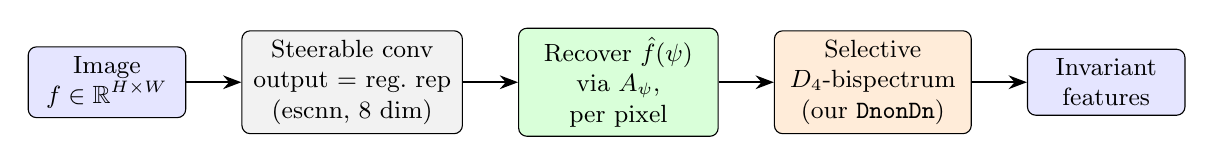
\begin{tikzpicture}[
    box/.style={draw, rounded corners=3pt, minimum height=0.8cm, font=\small, align=center},
    >=Stealth,
    node distance=0.6cm
  ]
    \node[box, fill=blue!10, minimum width=2cm] (img) {Image\\$f \in \R^{H \times W}$};
    \node[box, fill=gray!10, right=0.7cm of img, minimum width=2.8cm] (conv) {Steerable conv\\output = reg.\ rep\\(escnn, 8 dim)};
    \node[box, fill=green!15, right=0.7cm of conv, minimum width=2.5cm, text width=2.3cm] (fourier) {Recover $\hat{f}(\psi)$\\via $A_\psi$, per pixel};
    \node[box, fill=orange!15, right=0.7cm of fourier, minimum width=2.5cm] (bisp) {Selective\\$D_4$-bispectrum\\(our \texttt{DnonDn})};
    \node[box, fill=blue!10, right=0.7cm of bisp, minimum width=2cm] (out) {Invariant\\features};

    \draw[->, thick] (img) -- (conv);
    \draw[->, thick] (conv) -- (fourier);
    \draw[->, thick] (fourier) -- (bisp);
    \draw[->, thick] (bisp) -- (out);
  \end{tikzpicture}

  \bigskip

  \begin{itemize}
    \item \textbf{Steerable conv}: \texttt{escnn} with output type $A_1 \oplus A_2 \oplus B_1 \oplus B_2 \oplus 2E$ (regular-rep fiber, 8 scalars/pixel)
    \item \textbf{Fourier extraction}: invert $A_\psi$ to recover $\hat{f}(\psi)$ from each isotypic block (P4)
    \item \textbf{Selective bispectrum}: use our \texttt{DnonDn} module per pixel
    \item \textbf{Output}: $D_4$-invariant feature maps, ready for downstream task
  \end{itemize}

  \medskip

  Drop-in replacement for norm/gated nonlinearities in equivariant architectures.
\end{frame}

\begin{frame}{Experiment 1: rotated CIFAR-10/100}\small
  \textbf{Setup}: Standard benchmark for rotation-invariant classification.

  \medskip

  \begin{center}\scriptsize
  \begin{tabular}{llll}
    \toprule
    \textbf{Method} & \textbf{Invariance} & \textbf{Complete?}$^\dagger$ & \textbf{Source} \\
    \midrule
    Standard CNN + augmentation & None (learned) & N/A & Baseline \\
    Steerable CNN + norm & $D_4$ & No & Weiler \& Cesa 2019 \\
    Steerable CNN + $\SO(2)$ bisp. & $\SO(2)$ & Yes (rot) & Oreiller 2020 \\
    \textbf{Steerable CNN + $D_4$ sel.\ bisp.} & \textbf{$D_4$} & \textbf{Yes (rot+ref)} & \textbf{Ours} \\
    \multicolumn{4}{l}{\tiny $^\dagger$Generically, under non-degeneracy of relevant Fourier blocks.} \\
    \bottomrule
  \end{tabular}
  \end{center}

  \medskip

  \textbf{Expected}: $D_4$ selective bispectrum yields a generically complete invariant for rotations and reflections; norm is $D_4$-invariant too, but incomplete. Selective version matches full bispectrum with $8\times$ fewer channels.

  \medskip

  \textbf{Why impactful}: First head-to-head comparison of bispectrum vs norm/gate nonlinearities in steerable CNNs.
\end{frame}

\begin{frame}{Experiment 2: medical image segmentation}\small
  \textbf{Setup}: Reproduce Oreiller et al.\ (MIDL 2022) on MoNuSeg (nucleus segmentation in histopathology). Replace their $\SO(2)$ bispectral U-Net with our $D_4$ selective bispectral U-Net.

  \medskip

  \textbf{Why $D_4$ matters here}:
  \begin{itemize}\setlength{\itemsep}{1pt}
    \item Cell nuclei have no preferred chirality $\Rightarrow$ reflection invariance is natural
    \item $\SO(2)$ bispectrum handles rotations only
    \item $D_4$ bispectrum handles rotations \textit{and} reflections
  \end{itemize}

  \medskip

  \textbf{Expected}: Better rotation+reflection robustness on their benchmark, same architecture.

  \medskip

  \textbf{Why impactful}: Direct improvement on published results, on their own data, with a principled mathematical upgrade.
\end{frame}

\begin{frame}{Experiment 3: scaling analysis}\small
  How does the invariant feature dimension scale with group size?

  \vspace{-2pt}
  \centering
  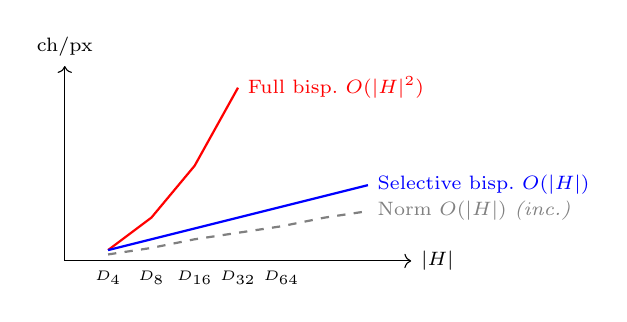
\begin{tikzpicture}[scale=0.55]
    \draw[->] (0,0) -- (8,0) node[right] {\scriptsize $|H|$};
    \draw[->] (0,0) -- (0,4.5) node[above] {\scriptsize ch/px};

    \draw[thick, red] (1,0.25) -- (2,1.0) -- (3,2.2) -- (4,4.0);
    \node[red, right, font=\scriptsize] at (4,4.0) {Full bisp.\ $O(|H|^2)$};

    \draw[thick, blue] (1,0.25) -- (2,0.5) -- (3,0.75) -- (4,1.0) -- (5,1.25) -- (6,1.5) -- (7,1.75);
    \node[blue, right, font=\scriptsize] at (7,1.75) {Selective bisp.\ $O(|H|)$};

    \draw[thick, gray, dashed] (1,0.15) -- (2,0.3) -- (3,0.5) -- (4,0.65) -- (5,0.8) -- (6,1.0) -- (7,1.15);
    \node[gray, right, font=\scriptsize] at (7,1.15) {Norm $O(|H|)$ \textit{(inc.)}};

    \foreach \x/\lab in {1/$D_4$, 2/$D_8$, 3/$D_{16}$, 4/$D_{32}$, 5/$D_{64}$} {
      \node[below, font=\tiny] at (\x, 0) {\lab};
    }
  \end{tikzpicture}

  \vspace{-2pt}
  \raggedright

  \textbf{Selective bispectrum} is the only option that is both:
  \begin{itemize}\setlength{\itemsep}{0pt}
    \item \textbf{Generically complete} (unlike norm, which loses phase)
    \item \textbf{Tractable} (unlike full bispectrum, which blows up quadratically)
  \end{itemize}

  \smallskip

  {\footnotesize Selectivity becomes increasingly important in 3D, where full bispectral constructions scale poorly with harmonic bandwidth.}
\end{frame}

\begin{frame}{Takeaway}\small
  \begin{enumerate}\setlength{\itemsep}{4pt}
    \item \textbf{Abelian steerable bispectrum} ($\SO(2)$) works: same scalar triple-product as \texttt{CnonCn}, applied per-pixel to circular-harmonic responses.

    \item For \textbf{non-abelian groups} ($D_n$, $O$), a single output type does not expose Fourier data for all irreps. Fix: \textbf{regular-representation output fiber}.

    \item \textbf{Proposition P4} (proved for $V = \C[H]$): $T_\psi(f) = (I_\psi \otimes A_\psi)\hat{f}(\psi)$. Multiplicity $d_\psi$ in output needed for $d_\psi$-dim irreps. Selectivity transfers.

    \item \textbf{Design}: for $D_4$, output $= A_1 \oplus A_2 \oplus B_1 \oplus B_2 \oplus 2E$ (8 scalars $= |D_4|$).

    \item \textbf{Target}: NeurIPS 2026. Theory + \texttt{SteerableBispectrum} layer + experiments on rotated CIFAR and MoNuSeg.
  \end{enumerate}

  \medskip

  \textbf{Remaining work}: map this construction to \texttt{escnn} --- verify the fiber can be set to the regular rep and compute $A_\psi$ from the intertwiner basis.
\end{frame}

\end{document}
